\documentclass[11pt,a4paper]{article}

\usepackage[utf8]{inputenc}
\usepackage[T1]{fontenc}
\usepackage[spanish]{babel}
\usepackage{amsmath}
\usepackage{amsfonts}
\usepackage{amssymb}
\usepackage{graphicx}
\usepackage{tabularx}
\usepackage{booktabs}
\usepackage{hyperref}
\usepackage{geometry}
\usepackage{listings}
\usepackage{xcolor}
\usepackage{caption}
\usepackage{subcaption}
\usepackage{titlesec}
\usepackage{parskip}
\usepackage{float}

% Configuración de títulos de párrafos
\titleformat{\paragraph}[hang]
{\normalfont\normalsize\bfseries}{\theparagraph}{1em}{}
\titlespacing*{\paragraph}
{0pt}{3.25ex plus 1ex minus .2ex}{1em}

\geometry{top=3cm, bottom=3cm, left=2.5cm, right=2.5cm}

\hypersetup{
    colorlinks=true,
    linkcolor=black,
    filecolor=magenta,      
    urlcolor=cyan,
}

\definecolor{codegreen}{rgb}{0,0.6,0}
\definecolor{codegray}{rgb}{0.5,0.5,0.5}
\definecolor{codepurple}{rgb}{0.58,0,0.82}
\definecolor{backcolour}{rgb}{0.95,0.95,0.92}

\lstdefinestyle{mystyle}{
    backgroundcolor=\color{backcolour},   
    commentstyle=\color{codegreen},
    keywordstyle=\color{magenta},
    numberstyle=\tiny\color{codegray},
    stringstyle=\color{codepurple},
    basicstyle=\ttfamily\small,
    breakatwhitespace=false,         
    breaklines=true,                 
    captionpos=b,                    
    keepspaces=true,                 
    numbers=left,                    
    numbersep=5pt,                  
    showspaces=false,                
    showstringspaces=false,
    showtabs=false,                  
    tabsize=2
}

\lstset{style=mystyle}

\begin{document}
\begin{titlepage}
    \begin{center}
        \vspace*{1cm}

        \Huge
        \textbf{Trabajo Practico N°1}

        \vspace{0.5cm}
        \LARGE
        Python

        \vspace{1.5cm}

        \vfill

        \Large
        \textbf{Autor:} Simón Saillen

        \Large
        \textbf{Profesores:} Ariel Pola, Agustin Pesce

        \vspace{0.5cm}

        \Large
        \textbf{Fundación Fulgor}\\
        Mayo 2026

    \end{center}
\end{titlepage}
\newpage

\section{Introducción}

En este trabajo práctico se trabaja con un filtro de coseno realzado (Raised
Cosine) en Python, integrando conceptos de comunicación serie y visualización
de señales tanto en el dominio temporal como frecuencial.

Se desarrollo un script interactivo (\texttt{filter\_by\_console.py}) que
permite crear filtros, visualizar su respuesta y consultar sus coeficientes a
través de una interfaz por consola que utiliza comunicación serie, simulando el
control de un dispositivo remoto mediante un puerto serial.

Además, se generaron diversas gráficas para analizar el comportamiento del
filtro: distintos factores de roll-off $\alpha$, agrupando respuestas
temporales y frecuenciales en una misma figura y contrastando las variantes RC
y RRC.\@

\section{Objetivos}

Los objetivos planteados para este trabajo fueron:

\begin{itemize}
    \item Utilizar un filtro de coseno realzado y raíz de coseno realzado dado por la
          fundación.
    \item Configurar los atributos del filtro mediante comandos enviados por puerto
          serie.
    \item Controlar el script a través del mismo puerto serie, tanto las funciones que
          generan el filtro como los métodos de la clase.
    \item Generar gráficas que muestren:
          \begin{itemize}
              \item Respuestas de varios filtros en un mismo ploteo.
              \item Respuesta en frecuencia y temporal agrupadas en una misma gráfica.
              \item Respuesta discreta utilizando \texttt{stem}.
          \end{itemize}
    \item Documentar el trabajo en un informe en formato \LaTeX.
\end{itemize}

\section{Desarrollo}

\subsection{Material proporcionado}

Se proporcionaron tres archivos base:

\begin{itemize}
    \item \texttt{filtro.py}: contiene la clase \texttt{RaisedCosineFilter}, que implementa un filtro de coseno realzado (RC) y raíz de coseno realzado (RRC). \\
          La clase tambien incluye metodos para plotear la respuesta temporal y frecuencial del filtro y obtener sus coeficientes.
    \item \texttt{com\_serie.py}: ejemplo de comunicación serie mediante \texttt{pySerial} en modo loopback, que envía y recibe datos carácter por carácter.
    \item \texttt{plot\_example.py}: ejemplo demostrativo de distintos tipos de gráficos usando \texttt{matplotlib}.
\end{itemize}

\subsection{Script \texttt{filter\_by\_console.py}}

Sobre la base de estos archivos, se desarrolló el script principal. Este
implementa una interfaz interactiva que permite:

\begin{itemize}
    \item Crear un filtro ingresando los parámetros por teclado. Internamente, se
          codifican y transmiten carácter por carácter por el puerto serie, replicando la
          mecánica de \texttt{com\_serie.py}.
    \item Visualizar la respuesta del filtro en tiempo y/o frecuencia utilizando el
          método \texttt{plot()} de la clase \texttt{RaisedCosineFilter}.
    \item Consultar los coeficientes del filtro generado.
\end{itemize}

El script expone un menú de comandos que el usuario puede ingresar:
\texttt{filter}, \texttt{plot}, \texttt{coef} y \texttt{exit}. Cada comando
activa un método distinto de la clase \texttt{ConsoleFilter}:

\begin{itemize}
    \item \texttt{filter}: solicita al usuario los parámetros del filtro
          ($\alpha$, \texttt{span}, \texttt{sps}, \texttt{rrc}). Cada uno de
          estos valores se codifica como cadena de texto y se transmite por el
          puerto serie carácter por carácter. Del otro lado del enlace se recibe el eco,
          se reconstruye el valor, y se instancia la clase
          \texttt{RaisedCosineFilter} con dichos parámetros.
    \item \texttt{plot}: solicita el tipo de gráfico (\texttt{time},
          \texttt{freq} o \texttt{both}), lo envía por serie y ejecuta el
          método \texttt{plot()} del filtro activo.
    \item \texttt{coef}: recupera e imprime los coeficientes del filtro mediante
          \verb|get_coefficients()|.
\end{itemize}

Cabe destacar que el script mantiene una única instancia activa del filtro a la
vez. Al usar el comando \texttt{filter} se crea una nueva instancia que
reemplaza a la anterior. Los comandos \texttt{plot} y \texttt{coef} operan
siempre sobre la última instancia creada, conservándola en memoria hasta que se
genere una nueva.

\section{Resultados}

A continuación se presentan las gráficas obtenidas a partir de la clase
\texttt{RaisedCosineFilter}.

\begin{figure}[H]
    \centering
    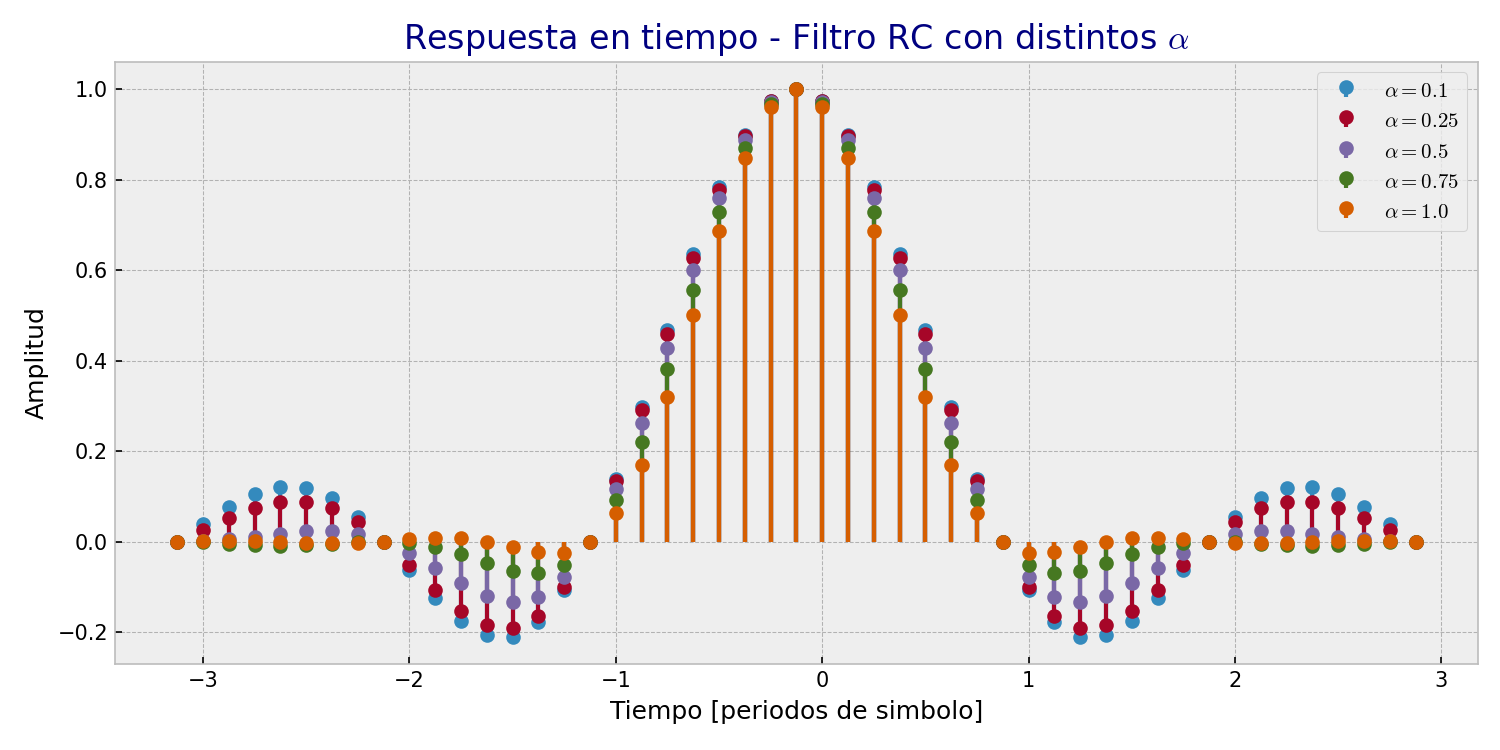
\includegraphics[width=0.85\textwidth]{../images/varios_filtros_time.png}
    \caption{Respuesta en tiempo de filtros RC con distintos valores de $\alpha$.}\label{fig:varios_time}
\end{figure}

Se observa cómo el factor de roll-off $\alpha$ afecta la forma de estos
coeficientes. Cuando $\alpha$ es pequeño ($\alpha=0.1$), los lóbulos laterales
son más pronunciados y de mayor amplitud. A medida que $\alpha$ aumenta, la
forma se vuelve más suave y los lóbulos laterales se atenúan, a costa de ocupar
más ancho de banda. Se nota que $\alpha=1.0$ presenta la curva más limpia y con
menor sobrepico.

\begin{figure}[H]
    \centering
    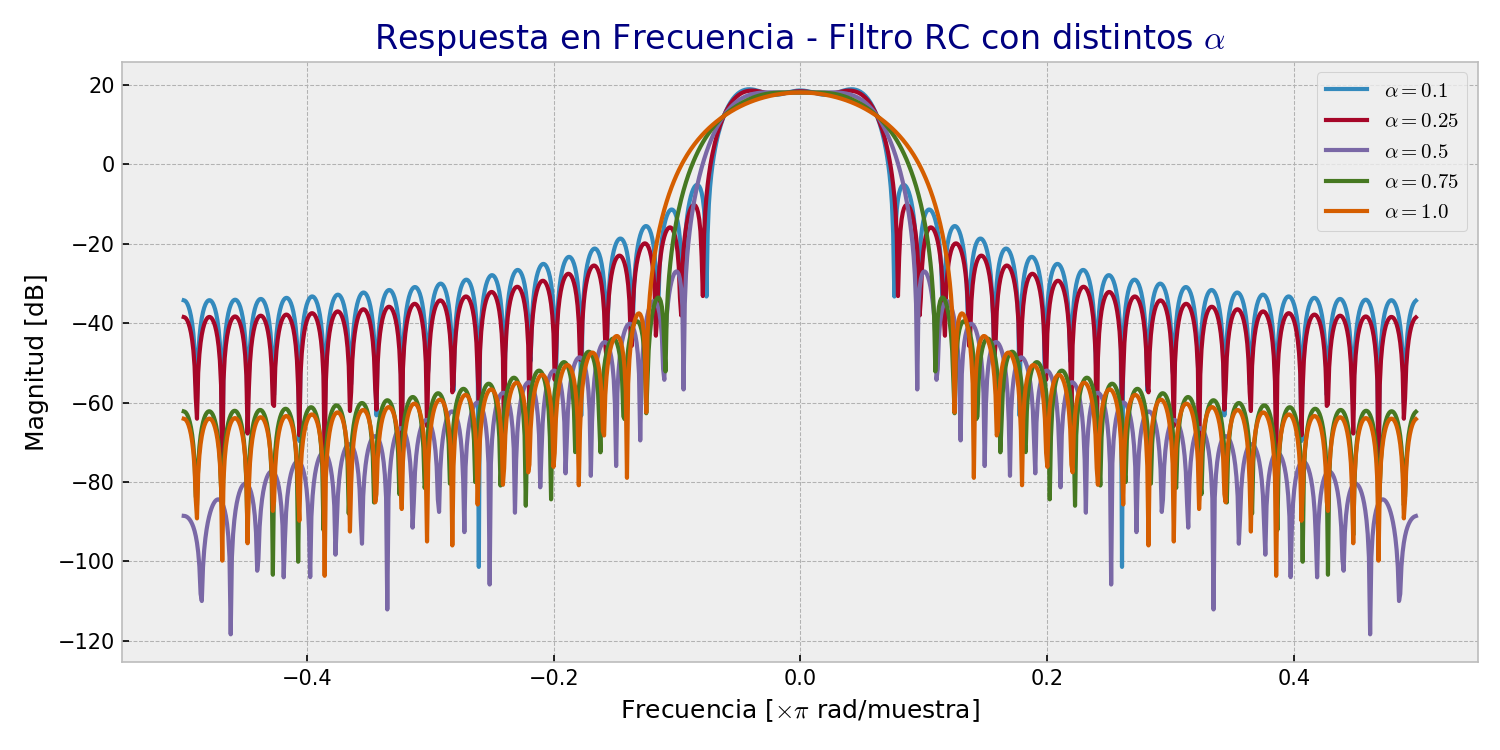
\includegraphics[width=0.85\textwidth]{../images/varios_filtros_freq.png}
    \caption{Respuesta en frecuencia de filtros RC con distintos valores de $\alpha$.}\label{fig:varios_freq}
\end{figure}

En frecuencia se observa claramente cómo $\alpha$ gobierna la pendiente de la
transición entre la banda de paso y la banda atenuada. Para $\alpha=0.1$ la
caída en la frecuencia de corte es casi vertical pero como se vio en la figura
anterior esto produce lóbulos laterales más pronunciados en tiempo. En cambio,
para $\alpha=1.0$ la transición es gradual y ocupa todo el ancho de banda
disponible, resultando en un mejor filtro temporal.

\begin{figure}[H]
    \centering
    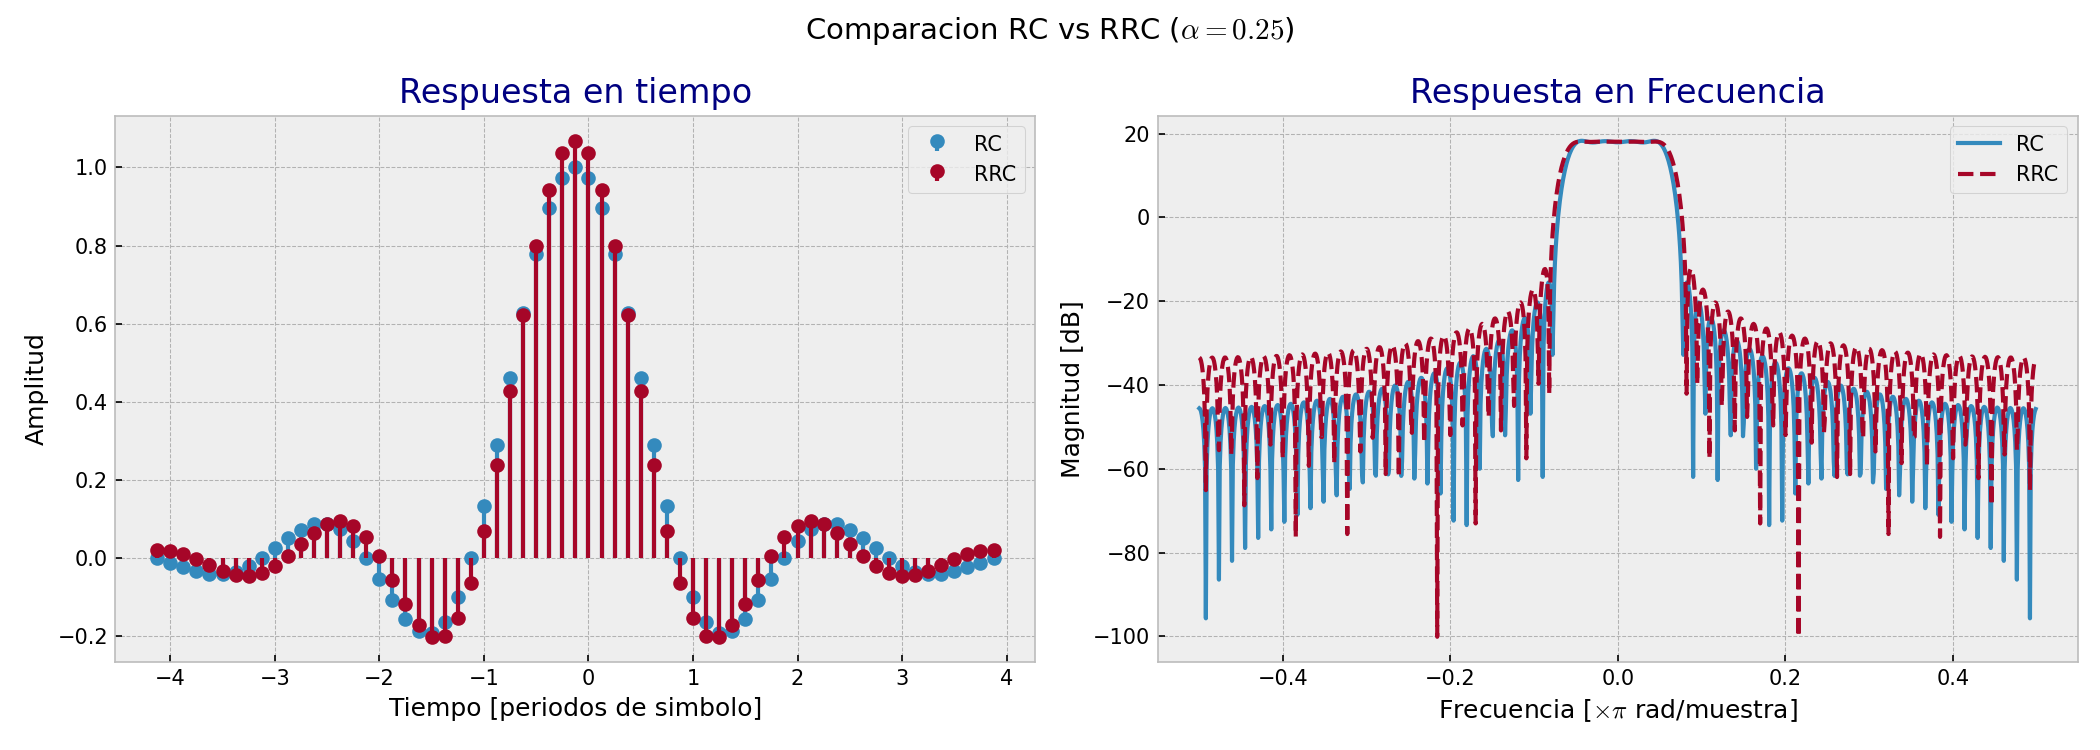
\includegraphics[width=0.85\textwidth]{../images/rc_vs_rrc.png}
    \caption{Comparación entre el filtro RC y RRC con $\alpha=0.25$.}\label{fig:rc_vs_rrc}
\end{figure}

La comparativa temporal revela que el filtro RRC posee una respuesta más
extendida y con mayor concentración de energía en sus extremos que el RC. En
frecuencia, si bien sus bandas de paso son análogas, el RRC demuestra un menor
desempeño en la banda de rechazo al exhibir un piso de lóbulos laterales de
aproximadamente -35 dB, en contraste con los -45 dB logrados por el RC.

\section{Conclusiones}

En este trabajo práctico se logró desarrollar e implementar con éxito el script
interactivo para el control y la configuración de filtros mediante comunicación
serie en modo loopback. El sistema demostró un funcionamiento robusto al
procesar correctamente la transmisión de comandos carácter por carácter,
permitiendo la actualización dinámica de los parámetros del filtro y la
consulta de sus coeficientes directamente desde la consola.

Respecto al análisis de los filtros, las gráficas obtenidas reflejan de manera
general el comportamiento esperado para cada configuración. Se constató que
variaciones en el factor de \textit{roll-off} ($\alpha$) modifican directamente
la pendiente de transición en frecuencia y la amplitud de los lóbulos en el
tiempo. Asimismo, la comparativa directa permitió verificar que el filtro RRC
presenta una respuesta temporal más dispersa hacia los extremos y una menor
atenuación fuera de la banda de paso en comparación con el filtro RC. En
conjunto, las herramientas de software y los métodos de visualización
implementados cumplieron con todos los objetivos prácticos planteados en la
consigna.

\end{document}